\documentclass{article}
\usepackage[UTF8]{ctex}
\usepackage{amsmath,amssymb}
\usepackage{tikz}
\usetikzlibrary{decorations.pathmorphing}
\usepackage{graphicx}
\usepackage{geometry}
\geometry{a4paper, margin=1in}

\begin{document}

\title{普通物理学学习笔记}
\author{Kaaovo}
\date{}
\maketitle

\tableofcontents

\section{切向加速度与法向加速度}

\subsection{切向（tangential）与法向（radial）加速度}
\begin{equation}
a_t = \frac{dv}{dt} = r \frac{d\omega}{dt} = r\alpha
\end{equation}
\begin{equation}
a_r = \frac{v^2}{r} = r\omega^2 \quad (\text{向心加速度})
\end{equation}
\begin{equation}
a = r\sqrt{\alpha^2 + \omega^4}
\end{equation}

\begin{center}
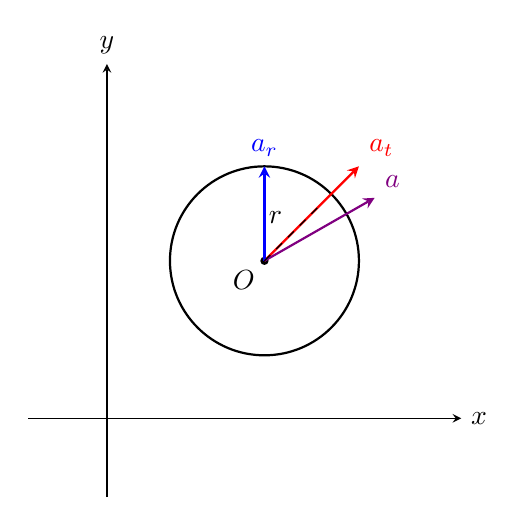
\begin{tikzpicture}[scale=1.0,>=stealth]
\draw[->] (-1,0) -- (4.5,0) node[right] {$x$};
\draw[->] (0,-1) -- (0,4.5) node[above] {$y$};
\draw[thick] (2,2) circle (1.2);
\fill (2,2) circle (1.5pt) node[below left] {$O$};
\draw[->,red,thick] (2,2) -- (3.2,3.2) node[above right] {$a_t$};
\draw[->,blue,thick] (2,2) -- (2,3.2) node[above] {$a_r$};
\draw[->,violet,thick] (2,2) -- (3.4,2.8) node[above right] {$a$};
\draw[dashed] (2,2) -- (2.7,2.7) node[midway,above left] {$r$};
\end{tikzpicture}
\end{center}

\section{刚体转动的功与功率}

\begin{equation}
dW = \vec{F} \cdot d\vec{s} = r d\theta \cdot F \sin\varphi = \tau d\theta
\end{equation}

\textbf{瞬时功率（Instantaneous power）}：
\begin{equation}
P = \frac{dW}{dt} = \tau \frac{d\theta}{dt} = \tau \omega
\end{equation}
（类比 \( P = Fv \)）

\begin{equation}
\sum \tau = I\alpha = I \frac{d\omega}{dt} = I \frac{d\omega}{d\theta} \frac{d\theta}{dt} = I\omega \frac{d\omega}{d\theta}
\end{equation}
\begin{equation}
\Rightarrow \sum \tau d\theta = I\omega d\omega
\end{equation}
\begin{equation}
\Rightarrow dW = I\omega d\omega \quad \Rightarrow \quad W = \frac{1}{2} I\omega^2
\end{equation}

\begin{center}
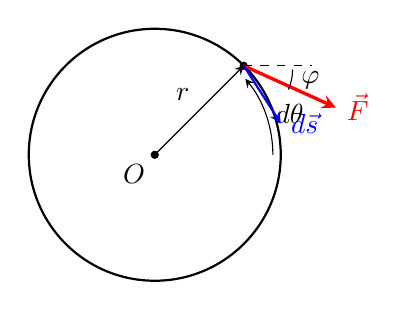
\begin{tikzpicture}[scale=1.0,>=stealth]
\draw[thick] (0,0) circle (1.6);
\fill (0,0) circle (1.5pt) node[below left] {$O$};
\draw[->] (0,0) -- (1.13,1.13) node[midway,above left] {$r$};
\fill (1.13,1.13) circle (1.5pt);
\draw[->,red,very thick] (1.13,1.13) -- (2.3,0.6) node[right] {$\vec{F}$};
\draw[dashed] (1.13,1.13) -- (2.0,1.13);
\draw (1.75,1.08) arc (0:-24:0.62) node[midway,right] {$\varphi$};
\draw[->] (1.5,0) arc (0:40:1.5) node[midway,right] {$d\theta$};
\draw[->,blue,thick] (1.13,1.13) -- (1.6,0.4) node[right] {$d\vec{s}$};
\end{tikzpicture}
\end{center}

\section{常见刚体的转动惯量}

\subsection{细杆绕中心（Rod about center）}
\begin{equation}
I = \int r^2 dm = \int_{-L/2}^{L/2} r^2 \cdot \frac{M}{L} dr = \frac{1}{12} ML^2
\end{equation}
（\( dm = \frac{M}{L} dr \)）

\begin{center}
\begin{tikzpicture}[scale=1.0,>=stealth]
\draw[very thick] (-2.5,0) -- (2.5,0);
\draw[->] (0,-0.3) -- (0,1.0) node[above] {转轴};
\node at (0,-0.5) {$O$};
\draw[<->] (-2.5,-0.5) -- (2.5,-0.5) node[midway,below] {$L$};
\draw[<->] (-2.5,0.3) -- (0,0.3) node[midway,above] {$L/2$};
\end{tikzpicture}
\end{center}

\subsection{细杆绕一端（Rod about one end）}
\begin{equation}
I = \int r^2 dm = \int_{0}^{L} r^2 \cdot \frac{M}{L} dr = \frac{1}{3} ML^2
\end{equation}

\begin{center}
\begin{tikzpicture}[scale=1.0,>=stealth]
\draw[very thick] (0,0) -- (4,0);
\draw[->] (0,-0.3) -- (0,1.0) node[above] {转轴};
\node at (0,-0.5) {$O$};
\draw[<->] (0,-0.5) -- (4,-0.5) node[midway,below] {$L$};
\end{tikzpicture}
\end{center}

\subsection{球壳（Spherical shell）}
\begin{equation}
I = \int r^2 dm = \int_0^\pi (R\sin\theta)^2 \frac{M \sin\theta d\theta}{2} = \frac{2}{3} MR^2
\end{equation}
（\( \dfrac{dm}{M} = \dfrac{2\pi R \sin\theta \cdot R d\theta}{4\pi R^2} = \dfrac{\sin\theta d\theta}{2} \)）

\begin{center}
\begin{tikzpicture}[scale=1.0,>=stealth]
\draw[thick] (0,0) circle (1.4);
\draw[->] (0,-1.6) -- (0,1.6) node[above] {转轴};
\draw[->] (0,0) -- (1.4,0) node[midway,above] {$R$};
\draw[dashed] (0,0) -- (0.99,0.99) node[midway,above left] {$r=R\sin\theta$};
\draw (0.35,0) arc (0:45:0.35) node[midway,right] {$\theta$};
\fill (0.99,0.99) circle (1.2pt);
\end{tikzpicture}
\end{center}

\subsection{实心球（Solid sphere）}
\begin{equation}
I = \int \frac{2}{3} r^2 dm = \int_0^R \frac{2}{3} r^2 \cdot \frac{3Mr^2}{R^3} dr = \frac{2}{5} MR^2
\end{equation}
（\( dm = \rho \cdot 4\pi r^2 dr = \dfrac{3Mr^2}{R^3} dr \)，球壳 \( dI = \frac{2}{3}r^2 dm \)）

\begin{center}
\begin{tikzpicture}[scale=1.0,>=stealth]
\draw[thick] (0,0) circle (1.4);
\draw[->] (0,-1.6) -- (0,1.6) node[above] {转轴};
\draw[->] (0,0) -- (1.4,0) node[midway,above] {$R$};
\draw[dashed] (0,0) circle (0.7);
\draw[->] (0,0) -- (0.7,0) node[midway,below] {$r$};
\end{tikzpicture}
\end{center}

\subsection{实心圆柱（Solid cylinder）}
\begin{equation}
I = \int r^2 dm = \int_0^R r^2 \cdot \frac{2Mr}{R^2} dr = \frac{1}{2} MR^2
\end{equation}
（\( dm = \dfrac{M}{\pi R^2 h} \cdot 2\pi r h dr = \dfrac{2Mr}{R^2} dr \)）

\begin{center}
\begin{tikzpicture}[scale=1.0,>=stealth]
\draw[thick] (0,-1.2) -- (0,1.2) node[above] {转轴};
\draw[thick] (0.8,0) ellipse (0.25 and 1.2);
\draw[thick] (-0.8,0) ellipse (0.25 and 1.2);
\draw[thick] (-0.8,-1.2) -- (0.8,-1.2);
\draw[thick] (-0.8,1.2) -- (0.8,1.2);
\draw[<->] (0.8,1.4) -- (0.8,1.9) node[above] {$R$};
\end{tikzpicture}
\end{center}

\section{平行轴定理（Parallel-Axis Theorem）}
\begin{equation}
I_P = I_{cm} + Md^2
\end{equation}
其中 \( d \) 为两平行轴间的距离。

\begin{center}
\begin{tikzpicture}[scale=1.0,>=stealth]
\draw[thick] (0,0) circle (1.2);
\fill (0,0) circle (1.5pt) node[below left] {$cm$};
\draw[->] (0,0) -- (0,1.6) node[above] {过质心轴};
\fill (2.2,0) circle (1.5pt);
\draw[->] (2.2,0) -- (2.2,1.6) node[above] {过 $P$ 轴};
\draw[<->] (0,-0.3) -- (2.2,-0.3) node[midway,below] {$d$};
\node at (2.2,-0.6) {$P$};
\end{tikzpicture}
\end{center}

\section{一些刚体模型}

\subsection{旋转杆（Rotating rod）}
长度 \( L \)，质量 \( M \)，均匀分布，绕一端转动。

由转动定律：
\begin{equation}
\tau = \frac{L}{2} \cdot Mg = I\alpha = \frac{1}{3} ML^2 \alpha
\end{equation}
\begin{equation}
\Rightarrow \alpha = \frac{3g}{2L}
\end{equation}
\begin{equation}
a_t = L \alpha = \frac{3}{2} g
\end{equation}

\begin{center}
\begin{tikzpicture}[scale=1.0,>=stealth]
\draw[very thick] (0,0) -- (3,0);
\fill (0,0) circle (1.5pt) node[left] {固定端 $O$};
\draw[->,red,very thick] (1.5,-0.2) -- (1.5,-1.2) node[below] {$Mg$};
\draw[->,blue,thick] (3,0.2) -- (3.8,0.6) node[right] {$a_t$};
\draw[<->] (0,0.4) -- (3,0.4) node[midway,above] {$L$};
\end{tikzpicture}
\end{center}

\section{滑轮转动（考虑滑轮半径 \( R \)、转动惯量 \( I \)，求加速度 \( a \)）}

\textbf{方法一（转动定律）}：
\begin{equation}
(T_1 - T_2) R = I\alpha = I \frac{a}{R}
\end{equation}
\begin{equation}
m_1 g - T_1 = m_1 a, \quad T_2 - m_2 g = m_2 a
\end{equation}
联立可解 \( T_1, T_2, a \)。

\textbf{方法二（能量守恒）}：
\begin{equation}
\Delta K + \Delta U = 0
\end{equation}
\begin{equation}
\Delta K = \frac{1}{2}(m_1+m_2) v^2 + \frac{1}{2} I \omega^2 = \frac{1}{2}\left( m_1 + m_2 + \frac{I}{R^2} \right) v^2
\end{equation}
\begin{equation}
\Delta U = (m_2 - m_1) g h
\end{equation}

\begin{center}
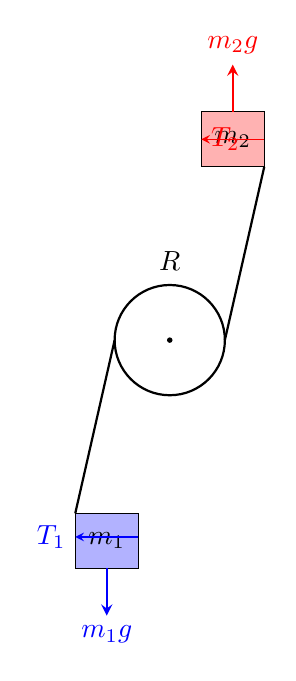
\begin{tikzpicture}[scale=1.0,>=stealth]
\draw[thick] (0,0) circle (0.7);
\fill (0,0) circle (1pt);
\node at (0,1.0) {$R$};
\draw[thick] (-0.7,0) -- (-1.2,-2.2);
\draw[thick] (0.7,0) -- (1.2,2.2);
\draw[fill=blue!30] (-1.2,-2.2) rectangle (-0.4,-2.9);
\node at (-0.8,-2.55) {$m_1$};
\draw[fill=red!30] (0.4,2.2) rectangle (1.2,2.9);
\node at (0.8,2.55) {$m_2$};
\draw[->,blue,thick] (-0.8,-2.9) -- (-0.8,-3.5) node[below] {$m_1 g$};
\draw[->,red,thick] (0.8,2.9) -- (0.8,3.5) node[above] {$m_2 g$};
\draw[->,blue] (-0.4,-2.5) -- (-1.2,-2.5) node[left] {$T_1$};
\draw[->,red] (1.2,2.55) -- (0.4,2.55) node[right] {$T_2$};
\end{tikzpicture}
\end{center}

\section{矢量式与参考系}

\begin{equation}
\vec{v} = \vec{\omega} \times \vec{r}, \quad \vec{\tau} = \vec{r} \times \vec{F}, \quad \vec{L} = \vec{r} \times \vec{p}
\end{equation}

\textbf{科里奥利力（Coriolis Force）}：\( -2m (\vec{\omega} \times \vec{v}_r) \)

\textbf{纯滚动（无滑动）}：
\begin{equation}
v_{cm} = \omega R
\end{equation}
接触点 \( P \) 的瞬时速度为零。

\begin{center}
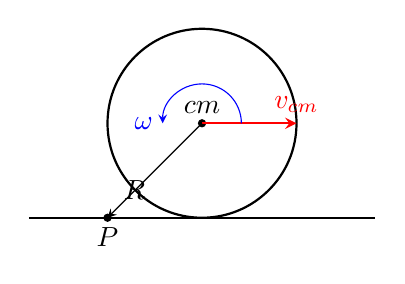
\begin{tikzpicture}[scale=1.0,>=stealth]
\draw[thick] (-2.2,-1.2) -- (2.2,-1.2);
\draw[thick] (0,0) circle (1.2);
\fill (0,0) circle (1.5pt) node[above] {$cm$};
\draw[->,red,thick] (0,0) -- (1.2,0) node[above] {$v_{cm}$};
\draw[->,blue] (0.5,0) arc (0:180:0.5) node[left] {$\omega$};
\fill (-1.2,-1.2) circle (1.5pt) node[below] {$P$};
\draw[->] (0,0) -- (-1.2,-1.2) node[midway,below left] {$R$};
\end{tikzpicture}
\end{center}

\section{角动量的应用}

\begin{equation}
\sum \vec{\tau}_{ext} = \frac{d\vec{L}}{dt}
\end{equation}
若 \( \sum \vec{\tau}_{ext} = 0 \)，则角动量守恒 \( \vec{L} = \text{const} \)。

\begin{equation}
\vec{L} = \sum \vec{r}_i \times (m_i \vec{v}_i), \quad L_z = I\omega
\end{equation}
\begin{equation}
\frac{dL_z}{dt} = I\alpha = \sum \tau_{ext,z}
\end{equation}
（注意一般 \( \vec{L} \neq I\vec{\omega} \)，仅当绕对称轴转动时成立。）

\textbf{例：子弹打杆}（子弹质量 \( m_d \)，杆质量 \( m_s \)，绕端点转动惯量 \( I \)）：
\begin{equation}
m_d V_{ai} = m_d V_{af} + m_s V_{s}
\end{equation}
\begin{equation}
-r m_d V_{ai} = -r m_d V_{af} - I\omega
\end{equation}
\begin{equation}
\frac{1}{2} m_d V_{ai}^2 = \frac{1}{2} m_d V_{af}^2 + \frac{1}{2} m_s V_s^2 + \frac{1}{2} I\omega^2
\end{equation}

\begin{center}
\begin{tikzpicture}[scale=1.0,>=stealth]
\draw[very thick] (0,0) -- (0,-3);
\fill (0,0) circle (1.5pt) node[above] {转轴 $O$};
\draw[fill=blue!40] (-0.25,-2.2) circle (0.25);
\node at (-0.6,-2.2) {$m_d$};
\draw[->,blue,thick] (-0.5,-2.2) -- (-1.6,-2.2) node[left] {$V_{ai}$};
\node at (0.4,-0.6) {$r$};
\draw[->,red,thick] (0.35,-2.2) -- (1.5,-2.2) node[right] {$V_{af}$};
\draw[->,violet,thick] (0,-1.5) arc (-90:-40:1.5) node[right] {$\omega$};
\end{tikzpicture}
\end{center}

\section{简谐振动（SHM）}

\begin{equation}
m \frac{d^2 x}{dt^2} = -kx \quad \Rightarrow \quad \frac{d^2 x}{dt^2} = -\omega^2 x, \quad \omega = \sqrt{\frac{k}{m}}
\end{equation}
\begin{equation}
x = A \cos(\omega t + \varphi)
\end{equation}
\begin{equation}
T = \frac{2\pi}{\omega}, \quad f = \frac{\omega}{2\pi}, \quad E = \frac{1}{2} kA^2
\end{equation}

\begin{center}
\begin{tikzpicture}[scale=1.0,>=stealth]
\draw[thick] (-3,0) -- (2.5,0);
\draw[fill=blue!30] (0.5,0.2) rectangle (1.3,0.9);
\node at (0.9,0.55) {$m$};
\draw[thick,decorate,decoration={coil,aspect=0.5,amplitude=2.5mm,segment length=2mm}] (-1.5,0.55) -- (0.5,0.55);
\fill (-1.5,0.55) circle (1.5pt);
\draw[thick] (-1.5,-0.2) -- (-1.5,1.3);
\draw[thick] (-3,-0.2) -- (-3,1.3) node[above] {墙};
\node at (-1.5,-0.5) {$k$};
\draw[<->] (1.3,1.0) -- (2.0,1.0) node[midway,above] {$x$};
\draw[dashed] (0,0) -- (0,-0.5) node[below] {平衡位置};
\end{tikzpicture}
\end{center}

\section{振动模型}

\subsection{单摆（Simple Pendulum）}
\begin{equation}
-mg \sin\theta = m L \frac{d^2 \theta}{dt^2}
\end{equation}
小角度时 \( \sin\theta \approx \theta \)：
\begin{equation}
\omega = \sqrt{\frac{g}{L}}, \quad \theta = \theta_0 \cos(\omega t + \varphi)
\end{equation}

\begin{center}
\begin{tikzpicture}[scale=1.0,>=stealth]
\fill (0,0) circle (1.5pt) node[above] {支点};
\draw[thick] (0,0) -- (1.5,-2.6);
\draw[fill=red!40] (1.5,-2.6) circle (0.25) node[right] {$m$};
\draw[dashed] (0,0) -- (0,-2.9);
\draw (0,-0.8) arc (-90:-60:0.8) node[midway,right] {$\theta$};
\draw[->,red,thick] (1.5,-2.6) -- (1.5,-3.4) node[below] {$mg$};
\draw[->,blue,thick] (1.5,-2.6) -- (1.1,-2.2) node[left] {$T$};
\node at (0.75,-1.3) {$L$};
\end{tikzpicture}
\end{center}

\subsection{物理摆（Physical Pendulum）}
\begin{equation}
\omega = \sqrt{\frac{mgd}{I}}
\end{equation}

\begin{center}
\begin{tikzpicture}[scale=1.0,>=stealth]
\fill (0,0) circle (1.5pt) node[above] {支点};
\draw[thick] (0,0) -- (1.5,-2.4);
\draw[fill=gray!30] (1.5,-2.4) circle (0.3);
\fill (1.5,-2.4) circle (1pt) node[right] {$cm$};
\draw[dashed] (0,0) -- (0,-2.7);
\draw (0,-0.8) arc (-90:-60:0.8) node[midway,right] {$\theta$};
\draw[->,red,thick] (1.5,-2.4) -- (1.5,-3.2) node[below] {$mg$};
\draw[<->] (0,-0.2) -- (1.5,-2.3) node[midway,above left] {$d$};
\end{tikzpicture}
\end{center}

\subsection{阻尼振动（Damped Oscillator）}
\begin{equation}
m\ddot{x} + b\dot{x} + kx = 0
\end{equation}
\begin{equation}
x = A e^{-\frac{b}{2m} t} \cos(\omega t + \varphi), \quad \omega = \sqrt{\frac{k}{m} - \left(\frac{b}{2m}\right)^2}
\end{equation}

\begin{center}
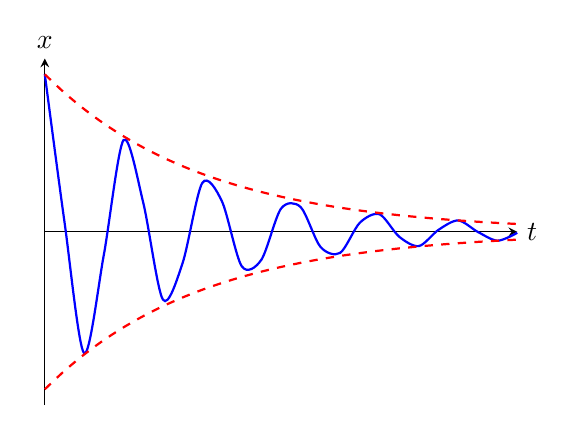
\begin{tikzpicture}[scale=1.0,>=stealth]
\draw[->] (0,0) -- (6,0) node[right] {$t$};
\draw[->] (0,-2.2) -- (0,2.2) node[above] {$x$};
\draw[blue,thick,domain=0:6,smooth,variable=\t] plot ({\t}, {2*exp(-0.5*\t)*cos(6*\t r)});
\draw[dashed,red,thick,domain=0:6,smooth] plot (\x,{2*exp(-0.5*\x)});
\draw[dashed,red,thick,domain=0:6,smooth] plot (\x,{-2*exp(-0.5*\x)});
\end{tikzpicture}
\end{center}

\subsection{简正模式（Normal Modes）}
两质量 \( m \) 由弹簧 \( k \) 相连，两端弹簧 \( k' \)：
\begin{equation}
\omega = \sqrt{\frac{k' + k}{m}} \ (\text{同相}), \quad \omega = \sqrt{\frac{k'}{m}} \ (\text{反相})
\end{equation}

\begin{center}
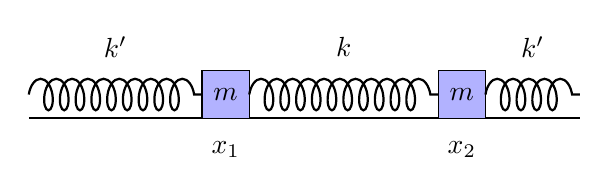
\begin{tikzpicture}[scale=1.0,>=stealth]
\draw[thick] (-1.5,0) -- (5.5,0);
\draw[fill=blue!30] (0.7,0) rectangle (1.3,0.6) node[midway] {$m$};
\draw[fill=blue!30] (3.7,0) rectangle (4.3,0.6) node[midway] {$m$};
\draw[thick,decorate,decoration={coil,aspect=0.5,amplitude=2mm,segment length=2mm}] (-1.5,0.3) -- (0.7,0.3);
\draw[thick,decorate,decoration={coil,aspect=0.5,amplitude=2mm,segment length=2mm}] (1.3,0.3) -- (3.7,0.3);
\draw[thick,decorate,decoration={coil,aspect=0.5,amplitude=2mm,segment length=2mm}] (4.3,0.3) -- (5.5,0.3);
\node at (-0.4,0.9) {$k'$};
\node at (2.5,0.9) {$k$};
\node at (4.9,0.9) {$k'$};
\node at (1,-0.4) {$x_1$};
\node at (4,-0.4) {$x_2$};
\end{tikzpicture}
\end{center}

\subsection{受迫振动与共振（Forced Oscillation）}
\begin{equation}
m\ddot{x} + b\dot{x} + kx = F_{ext}\cos(\omega t)
\end{equation}
共振时 \( \omega = \omega_0 = \sqrt{k/m} \)，振幅最大，相位差 \( \pi/2 \)。

\section{波}

\subsection{横波与纵波}

\begin{center}
\begin{tikzpicture}[scale=1.0,>=stealth]
\begin{scope}[yshift=1.2cm]
\draw[blue,thick,domain=0:6,smooth,variable=\x] plot (\x,{sin(\x r)});
\draw[->] (0,-1.2) -- (0,1.2);
\draw[->] (0.5,0.84) -- (0.5,1.6) node[above] {振动方向};
\draw[->] (0.5,0) -- (2.0,0) node[right] {传播方向};
\node at (3,-1.6) {横波（振动 $\perp$ 传播）};
\end{scope}
\begin{scope}[yshift=-2.5cm]
\foreach \x in {0,0.7,1.4,2.1,2.8,3.5,4.2,4.9,5.6} \draw[fill=blue!40] (\x,0) circle (0.15);
\draw[->] (0,0) -- (6,0) node[right] {传播方向};
\node at (3,-1.6) {纵波（振动 $\parallel$ 传播）};
\end{scope}
\end{tikzpicture}
\end{center}

\subsection{波动方程与波速}
\begin{equation}
\frac{\partial^2 y}{\partial t^2} = v^2 \frac{\partial^2 y}{\partial x^2}, \quad v = \frac{\omega}{k} = \frac{\lambda}{T}
\end{equation}

\subsection{弦上波速}
\begin{equation}
v = \sqrt{\frac{F}{\mu}}
\end{equation}
（\( F \) 为张力，\( \mu \) 为线密度）

\begin{center}
\begin{tikzpicture}[scale=1.0,>=stealth]
\draw[thick] plot[smooth] coordinates {(0,0) (1,0.7) (2,1.0) (3,0.7) (4,0)};
\draw[->,red,thick] (1.6,0.85) -- (0.9,1.3) node[above] {$F$};
\draw[->,red,thick] (1.6,0.85) -- (2.3,1.3) node[above] {$F$};
\draw[dashed] (1.6,0.85) -- (1.6,0) node[below] {$\Delta x$ 中点};
\end{tikzpicture}
\end{center}

\subsection{干涉}
\begin{equation}
\text{相长}: \Delta r = n\lambda, \qquad \text{相消}: \Delta r = (n + \tfrac{1}{2}) \lambda
\end{equation}
\textbf{拍频}：\( f_b = |f_1 - f_2| \)

\subsection{驻波（Standing waves）}
\begin{equation}
y = 2A \sin(kx) \cos(\omega t)
\end{equation}

\begin{center}
\begin{tikzpicture}[scale=1.0,>=stealth]
\draw[->] (0,0) -- (6.5,0);
\draw[blue,thick,domain=0:6.28,smooth,variable=\x] plot (\x,{sin(\x r)});
\draw[blue,thick,dashed,domain=0:6.28,smooth,variable=\x] plot (\x,{-sin(\x r)});
\foreach \x in {0,3.14,6.28} \fill (\x,0) circle (1.5pt) node[below] {波节};
\foreach \x in {1.57,4.71} \fill (\x,0) circle (1.5pt) node[above] {波腹};
\end{tikzpicture}
\end{center}

\section{声波与多普勒效应}

\subsection{声速与声强}
\begin{equation}
v = \sqrt{\frac{B}{\rho}}, \quad I = \frac{1}{2} B \omega k A^2
\end{equation}

\subsection{多普勒效应}
\begin{equation}
f' = \frac{v + v_o}{v - v_s} f
\end{equation}
\( v_o \)：观察者速度，\( v_s \)：波源速度（正方向约定从观察者指向波源）。

\begin{center}
\begin{tikzpicture}[scale=1.0,>=stealth]
\fill (-3,0) circle (2pt) node[left] {$S$ 波源};
\fill (3,0) circle (2pt) node[right] {$O$ 观察者};
\draw[->,blue,thick] (-3,0.4) -- (-3,1.2) node[above] {$v_s$};
\draw[->,red,thick] (3,0.4) -- (3,1.2) node[above] {$v_o$};
\draw[<->] (-2.6,-0.4) -- (2.6,-0.4) node[midway,below] {$v$（波速）};
\draw[->,thick] (-2.7,0) -- (2.7,0);
\end{tikzpicture}
\end{center}

\section{相对论}

\subsection{光速不变与速度合成}
\begin{equation}
w = \frac{u + v}{1 + \frac{uv}{c^2}}
\end{equation}

\subsection{时间膨胀与长度收缩}
\begin{equation}
\Delta t = \gamma \Delta t_0, \quad L = \frac{L_0}{\gamma}, \quad \gamma = \frac{1}{\sqrt{1 - v^2/c^2}}
\end{equation}

\subsection{洛伦兹变换}
\begin{equation}
x' = \gamma(x - vt), \quad t' = \gamma(t - \frac{vx}{c^2}), \quad y'=y, \ z'=z
\end{equation}

\subsection{光锥（Minkowski 图）}
\begin{center}
\begin{tikzpicture}[scale=1.0,>=stealth]
\draw[->] (0,-2.5) -- (0,2.5) node[above] {$ct$};
\draw[->] (-2.5,0) -- (2.5,0) node[right] {$x$};
\draw[red,thick] (-2.3,-2.3) -- (2.3,2.3);
\draw[red,thick] (-2.3,2.3) -- (2.3,-2.3);
\node[red] at (1.9,1.5) {光锥};
\node at (1.1,-1.3) {类时};
\node at (0.9,1.6) {类时};
\node at (1.7,0.4) {类空};
\node at (-1.7,0.4) {类空};
\end{tikzpicture}
\end{center}

\subsection{质能关系}
\begin{equation}
E = mc^2 = \gamma m_0 c^2, \quad E_0 = m_0 c^2, \quad E^2 = p^2 c^2 + m_0^2 c^4
\end{equation}
对光子：\( E = h\nu, \ p = h\nu/c \)。

\section{热学}

\subsection{热膨胀}
\begin{equation}
\Delta L = \alpha L_0 \Delta T, \quad \Delta V = \beta V_0 \Delta T, \quad \beta \approx 3\alpha
\end{equation}

\subsection{理想气体状态方程}
\begin{equation}
PV = nRT = N k_B T
\end{equation}
\textbf{范德瓦尔斯方程}：\( (P + \frac{an^2}{V^2})(V - nb) = nRT \)

\subsection{气体动理论}
\begin{equation}
P = \frac{1}{3} \rho \overline{v^2}, \quad \frac{1}{2} m \overline{v^2} = \frac{3}{2} k_B T
\end{equation}

\begin{center}
\begin{tikzpicture}[scale=1.0,>=stealth]
\draw[thick] (0,0) rectangle (4,3);
\draw[very thick] (4,0) -- (4,3);
\node at (4.3,1.5) {壁 $A$};
\draw[fill=red!40] (0.8,1.0) circle (0.15);
\draw[fill=blue!40] (1.6,2.2) circle (0.15);
\draw[fill=green!40] (2.4,0.8) circle (0.15);
\draw[fill=orange!40] (3.0,1.8) circle (0.15);
\draw[->,blue,thick] (1.6,2.2) -- (2.6,2.2) node[above] {$v_x$};
\draw[->,red] (0.8,1.0) -- (1.8,1.3);
\draw[->,green] (2.4,0.8) -- (3.2,0.5);
\node at (2,3.4) {体积 $V$，$N$ 个分子};
\end{tikzpicture}
\end{center}

\subsection{麦克斯韦速度分布}
\begin{equation}
f(v) = 4\pi \left( \frac{m}{2\pi k_B T} \right)^{3/2} v^2 e^{-\frac{mv^2}{2k_B T}}
\end{equation}

\begin{center}
\begin{tikzpicture}[scale=1.0,>=stealth]
\draw[->] (0,0) -- (5,0) node[right] {$v$};
\draw[->] (0,0) -- (0,2.5) node[above] {$f(v)$};
\draw[blue,thick,domain=0:4.8,smooth,variable=\v] plot ({\v},{1.6*(\v*\v)*exp(-\v*\v/2)});
\draw[dashed] (1.41,0) -- (1.41,1.18);
\draw[dashed] (1.73,0) -- (1.73,1.27);
\draw[dashed] (2,0) -- (2,1.3);
\node at (1.41,-0.3) {$v_p$};
\node at (1.73,-0.3) {$\bar{v}$};
\node at (2.2,-0.3) {$v_{rms}$};
\end{tikzpicture}
\end{center}

\section{热力学第一定律}

\begin{equation}
\Delta U = Q - W
\end{equation}

\subsection{等温、等压、等体过程}
\begin{equation}
W_{iso} = nRT \ln\frac{V_f}{V_i}, \quad C_p = C_v + R, \quad \gamma = \frac{C_p}{C_v}
\end{equation}

\subsection{绝热过程}
\begin{equation}
P V^\gamma = \text{const}, \quad T V^{\gamma - 1} = \text{const}
\end{equation}

\subsection{热机效率与卡诺循环}
\begin{equation}
e = \frac{W}{Q_H}, \quad e_{Carnot} = 1 - \frac{T_c}{T_h}
\end{equation}

\begin{center}
\begin{tikzpicture}[scale=1.0,>=stealth]
\draw[->] (0,0) -- (5,0) node[right] {$V$};
\draw[->] (0,0) -- (0,3.5) node[above] {$P$};
\draw[thick,red] plot[smooth] coordinates {(1.0,3.0) (2.2,1.8)};
\draw[thick,blue] plot[smooth] coordinates {(2.0,1.2) (3.4,0.7)};
\draw[thick,green!50!black] plot[smooth] coordinates {(1.0,3.0) (2.0,1.2)};
\draw[thick,orange] plot[smooth] coordinates {(2.2,1.8) (3.4,0.7)};
\node[red] at (1.5,2.6) {$Q_H$};
\node[blue] at (2.8,0.9) {$Q_L$};
\node at (1.5,1.4) {绝热};
\node at (2.8,1.4) {绝热};
\node at (1.9,2.1) {等温};
\node at (2.3,0.95) {等温};
\end{tikzpicture}
\end{center}

\end{document}
